\documentclass[11pt,letterpaper]{article}
\usepackage{fullpage}
\usepackage{multicol}
\usepackage{amsmath}
\usepackage{amsfonts}
\usepackage{amssymb}
\usepackage{graphicx}
%\usepackage{pstricks, pst-node, pst-plot}

\newcommand{\ds}{\displaystyle}
\newcommand{\bv}{\mathbf}
\newcommand{\lv}{\langle}
\newcommand{\rv}{\rangle}

\begin{document}
\flushleft
\begin{multicols}{2}


\begin{large}\textbf{Math 115 Quiz 7: $\oint $ 3.9, 4.1, 4.2 Using First and Second Derivatives \\
Mon 8 November 2010}\end{large}

\textbf{Name:  }\underline{\hspace{35ex}}

\vspace{.5in}

\end{multicols}

\pagestyle{empty}

\flushleft

You have 20 minutes to complete this quiz.  Make your variables clear and
consistent (so if you want to say, for example, $\frac{dy}{dx}$, you should also
mention $y=f(x)$, or ``$y$ is a function of $x$'').  Calculators are OK.  

\begin{enumerate}
\item \textbf{Definitions/Concepts.} 
\begin{enumerate}
 \item (2 pts) Complete this statement:  Suppose $f$ is differentiable at $a$.  Then, for values of $x$ near $a$, the tangent line approximation to $f(x)$ is
\[f(x)\approx f(a)+f'(a)(x-a).\]
 
\vspace{1pc}
\item (1 pt) TRUE or \textbf{FALSE}: If the derivative of $f$ is zero at the point $x=a$, then $a$ is either a local maximum or a local minimum.

\vspace{.5pc}
For example, if $f(x)=x^3$, then $f'(0)=0$.  However, $x=0$ is not a local maximum or a local minimum.
\end{enumerate}

\vspace{1pc}
\item \textbf{Questions/Problems.} (3 pts) For which powers $p$ is $y=x^p$ concave up on the
region $x\in (0,\infty)$?  Explain.

\vspace{.5pc}
First, look at the second derivative:
\begin{eqnarray*}
 y &=& x^p \\
y' &=& px^{p-1} \\
y'' &=& (p-1)px^{p-2}.
\end{eqnarray*}
Concave up means $y''>0$.  When $x\in (0,\infty )$, $x^{p-2}$ can never be negative.  So it is necessary to only look at when $(p-1)p>0$.  When $p$ and $p-1$ are both positive $p-1$ is smaller than $p$, so really we only need $p-1>0$.  This happens when $p>1$.  When $p$ and $p-1$ are both negative it is enough that $p<0$.  Hence, for all $p\in (-\infty ,0)\cup (1,\infty )$, $y=x^p$ is concave up on the domain $x\in (0,\infty )$.

\vspace{1pc}
\noindent (3 pts) Are exponential functions of the form $y=mc^t$
always increasing if $m>0$? If yes, say why. If no, give a
concrete counterexample (equation and sketch of graph).

\vspace{.5pc}
No.  For example, if $c=1$ then $y=m\cdot 1^t=m$ has the following constant graph:
\begin{center}
 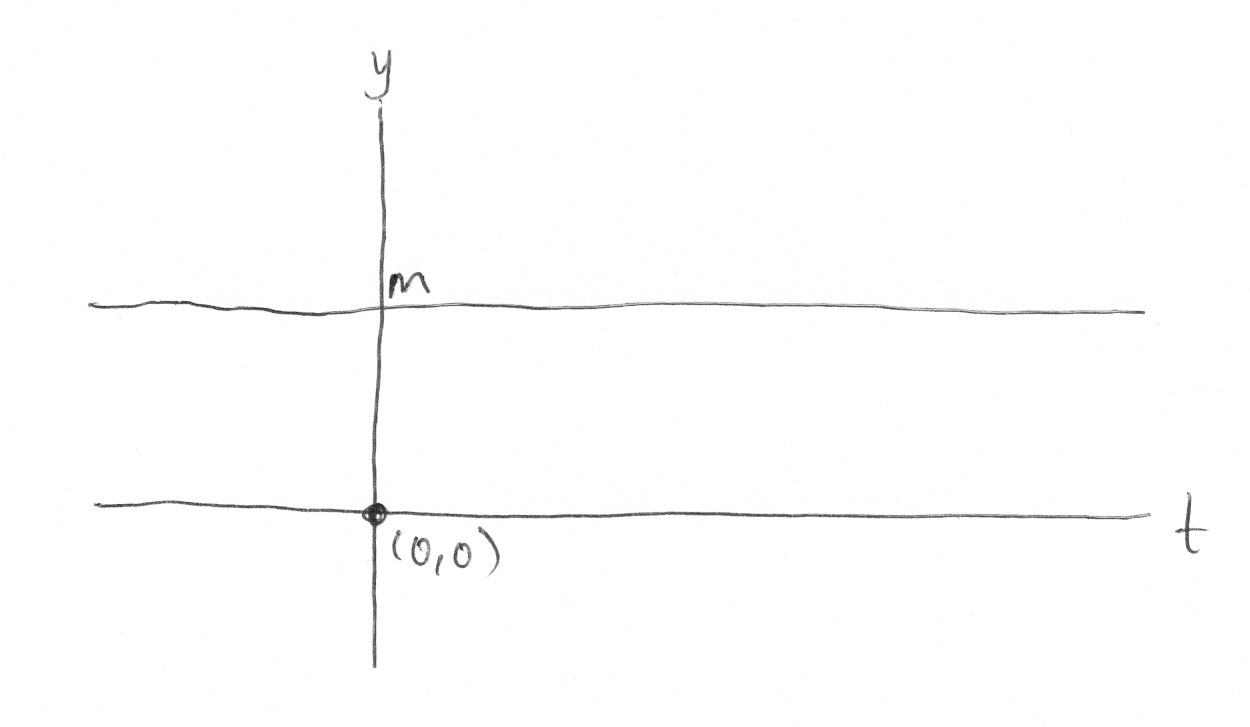
\includegraphics[scale=.4]{./quiz7pic.jpg}
\end{center}

%\begin{flushright}
% turn over $\rightarrow $
%\end{flushright}

\pagebreak
\item \textbf{Computations/Algebra.} (1 pt) Find all critical points of the following function.  Use the second derivative to tell if each critical point is a local maximum, local minimum, or cannot be determined. 
\[f(x)=(x^3-8)^4\]
\end{enumerate}
Critical points are where $f'=0$.
\begin{eqnarray*}
 f'(x)=0 &=& 4(x^3-8)^3\cdot (3x^2) \\
&=& 12x^2(x^3-8)^3
\end{eqnarray*}
So either $x=0$ or $x^3-8=0$.  Therefore the critical points are $x=0,2$.  The second derivative is
\begin{eqnarray*}
 f''(x) &=& 24x(x^3-8)^3+12x^2\cdot 3(x^3-8)^2\cdot (3x^2) \\
&=& 24x(x^3-8)^3+108x^3(x^3-8)^2.
\end{eqnarray*}
Substituting in the critical points,
\begin{eqnarray*}
f''(0) &=& 24(0)((0)^3-8)^3+108(0)^3((0)^3-8)^2 \\
&=& 0 
\end{eqnarray*}
means it cannot be determined if $x=0$ is an extremum.  Similarly,
\begin{eqnarray*}
f''(2) &=& 24(2)((2)^3-8)^3+108(2)^3((2)^3-8)^2 \\
&=& 0 
\end{eqnarray*}
so it cannot be determined if $x=2$ is an extremum.
%----------------------------------------------------------------------------------------

\vspace{1pc}
%\noindent \textbf{ChAlLeNgE PrObLeM:}  

\end{document}


